\paragraph*{}
Object recognition is a common task of computer vision for identifying a specific object in a digital image or video. Humans can recognize multiple objects in images with little effort, but this task is still a big challenge for computer vision systems due to the fact that the objects may vary somewhat in different view points, in many different sizes, scales, types or even when they are translated or rotated (in video). 

\begin{figure}[h!]
	\captionsetup{width=0.8\textwidth}
	\centering
	\begin{subfigure}[b]{0.2\linewidth}
		
\includegraphics[width=\linewidth]{images/chairs/0.jpeg}
	\end{subfigure}
	\begin{subfigure}[b]{0.2\linewidth}
		
\includegraphics[width=\linewidth]{images/chairs/1.jpeg}
	\end{subfigure}
	\begin{subfigure}[b]{0.2\linewidth}
		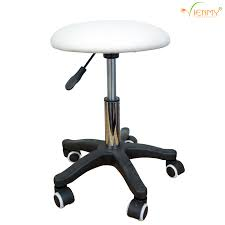
\includegraphics[width=\linewidth]{images/chairs/2.jpeg}
	\end{subfigure}
	
	\begin{subfigure}[b]{0.2\linewidth}
		
\includegraphics[width=\linewidth]{images/chairs/3.jpeg}
	\end{subfigure}
	\begin{subfigure}[b]{0.2\linewidth}
		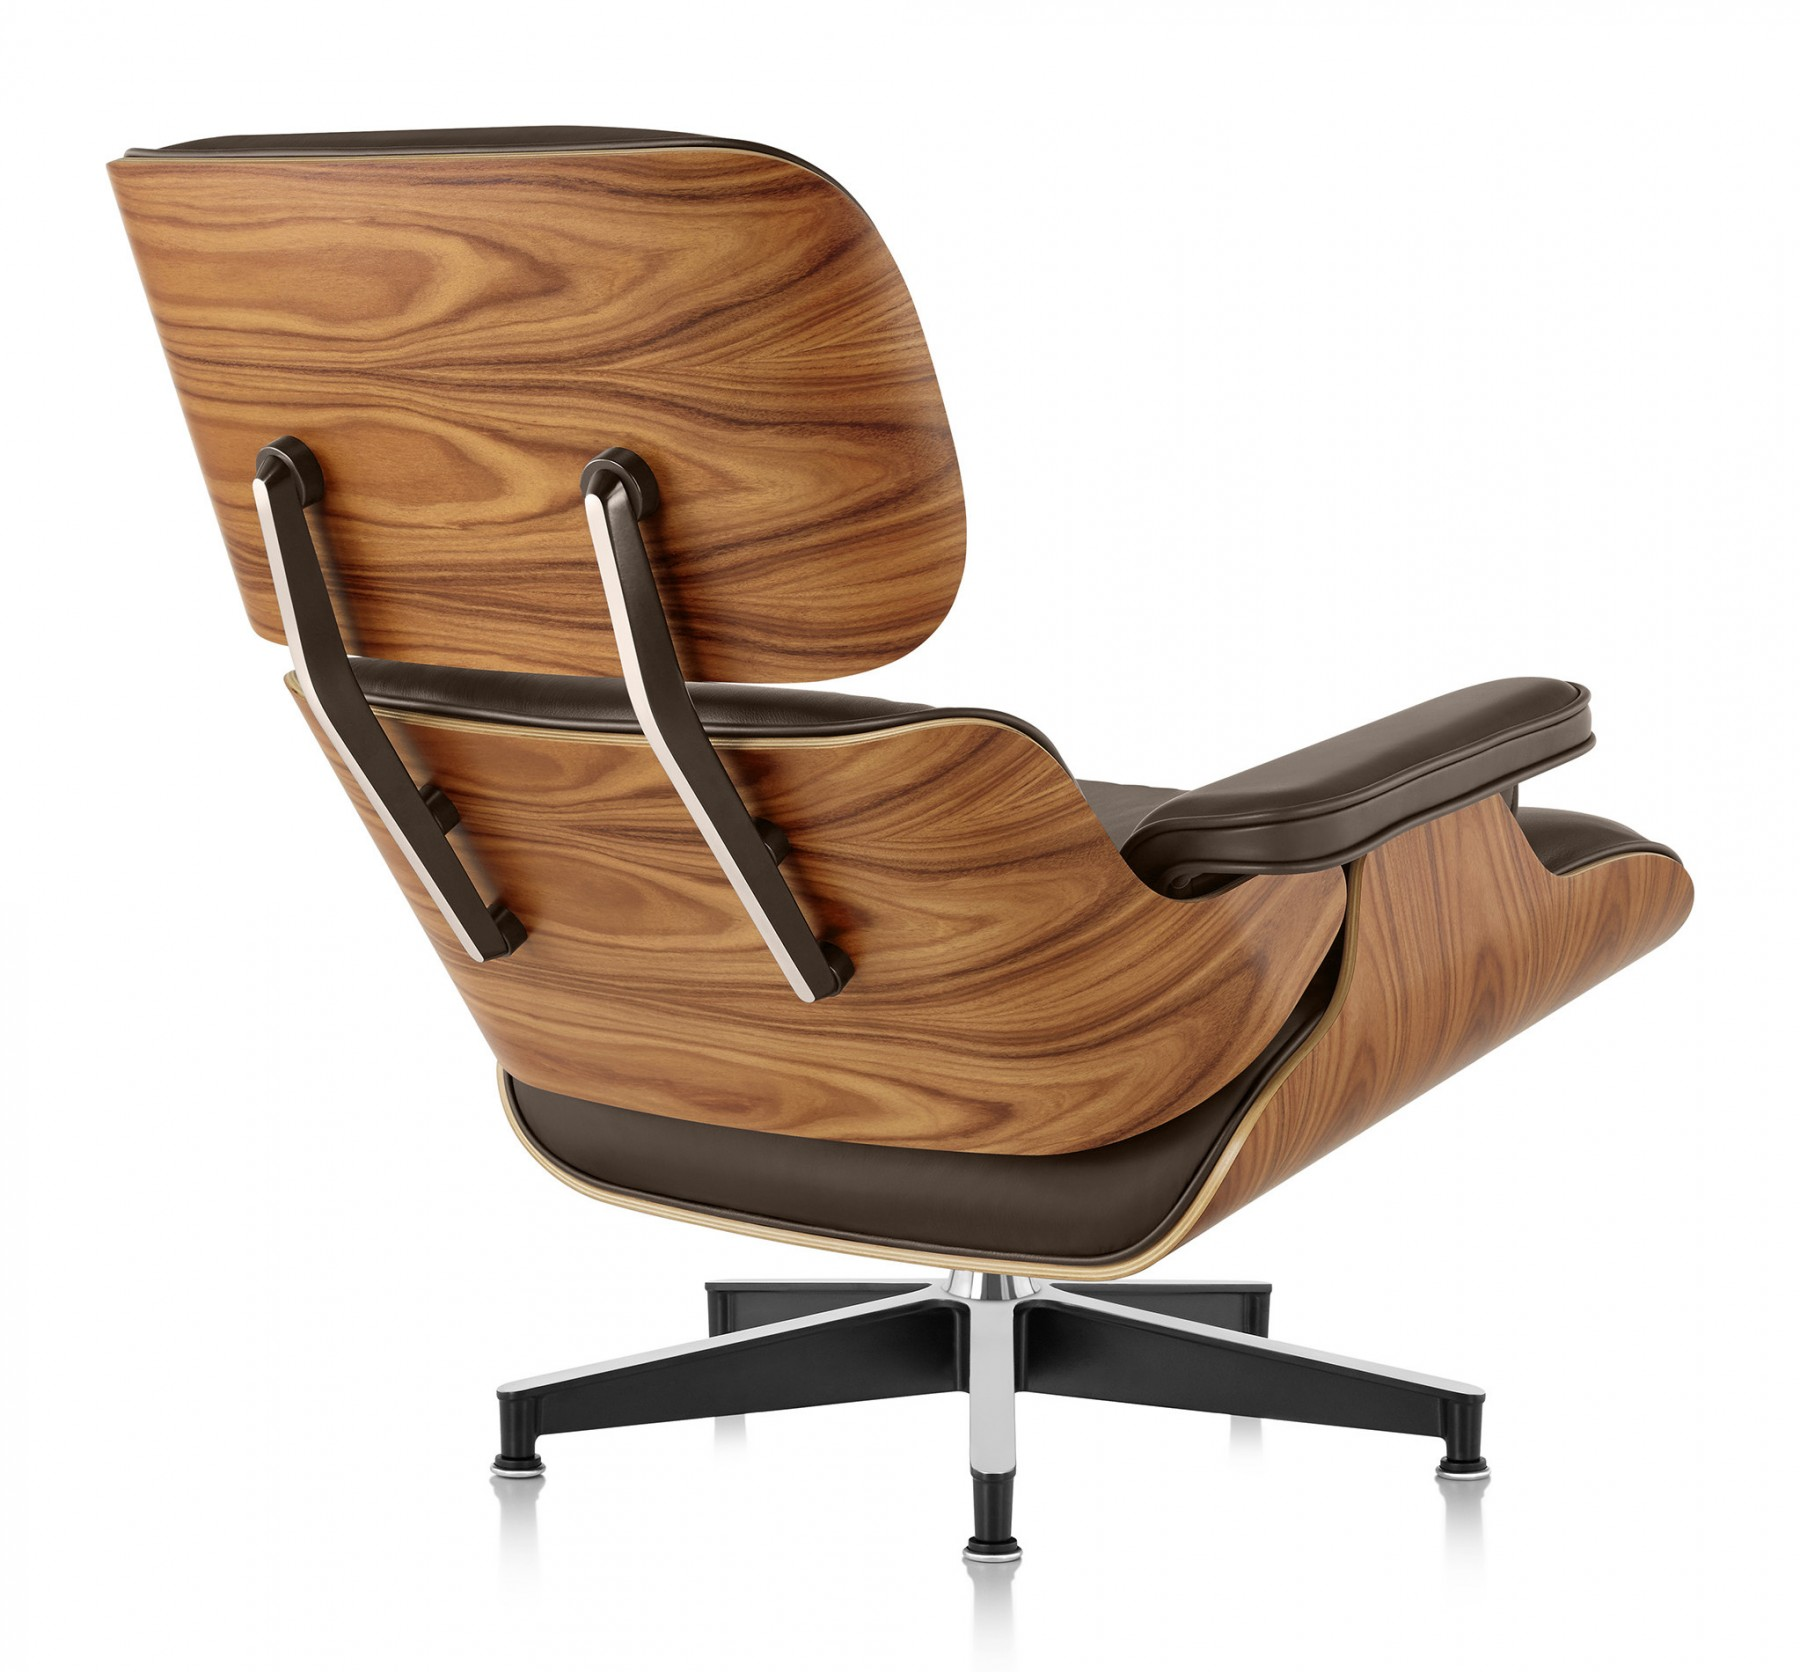
\includegraphics[width=\linewidth]{images/chairs/4.jpg}
	\end{subfigure}
	\begin{subfigure}[b]{0.2\linewidth}
		
\includegraphics[width=\linewidth]{images/chairs/5.jpg}
	\end{subfigure}
  	\caption[Object recognition challanges example]{Chairs with different view points, sizes, materials make the recognition task more challenging.}
\end{figure}

\paragraph*{}
Object recognition is useful in applications such as video stabilization \cite{ARTICLE:0}, Manufacturing Quality Control \cite{BOOK:0}, Automated vehicle parking systems \cite{BOOK:1}, etc. 

\paragraph*{}
Many approaches to the task have been implemented over the years. Common techniques include deep learning based approaches such as convolutional neural networks, and feature-based approaches using edges, gradients, histogram of oriented gradients (HOG), Haar wavelets, and linear binary patterns.

\paragraph*{}
In this project, we end up with a simple feature-based approache using Bag of words (BOW) with two different learning algorithms K-Nearest Neighbor (KNN) and Support Vector Machine (SVM) on Caltech101 just for practising what we have learn from the class.
